\subsection{Описание кода программной реализации}
Код реализации выложен на \mintinline{bash}{C++} в репозитории \cite{Repository}

\begin{figure}[ht]
    \centering
    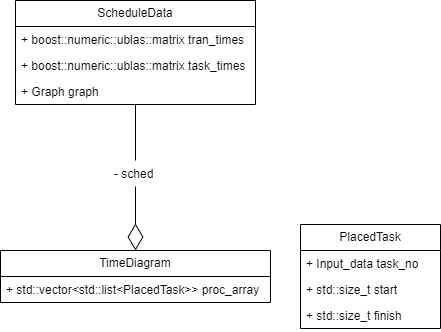
\includegraphics[width=0.8\textwidth]{imgs/final_UML.drawio.png}
    \caption{UML-диаграмма реализации}
    \label{fig:UML}
\end{figure}

Среди представленных классов:
\begin{itemize}
    \item \mintinline{C++}{ScheduleData} - класс, хранящий в себе входные данные и выполняющий всю необходимую их предобработку.
    \item \mintinline{C++}{TimeDiagram} - класс, хранящий в себе частичное или полное расписание.
    \item \mintinline{C++}{PlacedTask} - класс, хранящий в себе информацию о поставленной в расписание работе.
\end{itemize}

Жадные алгоритмы реализованы в функциях, не инкапсулированных в классах:
\begin{itemize}
    \item \mintinline{C++}{construct_time_schedule()} - жадный алгоритм с жадным критерием.
    \item \mintinline{C++}{greedy_EDF_heuristic()} - Жадный алгоритм с EDF эвристикой.
\end{itemize}

В репозиторий включены следубщие библиотеки:
\begin{enumerate}
    \item \mintinline{bash}{METIS} 5.1.0 \cite{METIS_lib} - библиотека для разбиения графов.
    \item \mintinline{bash}{json} 3.11.2 \cite{json_lib} - библиотека для работы с форматом JSON. Используется для составления выходных файлов.
    \item \mintinline{bash}{toml11} 3.7.1 \cite{toml11_lib} - библиотека для работы с форматом TOML. Используется для чтения конфигурационных файлов.
\end{enumerate}

Также, у реализации есть зависимость, не включенная в репозиторий - \mintinline{bash}{boost} 1.80 \cite{boost_framework}

Для сборки проекта используется \mintinline{bash}{CMake}.
\begin{minted}{bash}
    mkdir build
    cd build
    cmake ..
    make
\end{minted}

Для сборки документации (на английском) используется \mintinline{bash}{Doxygen}.
\begin{minted}{bash}
    doxygen Doxyfile
\end{minted}

\subsection{Описание интерфейса программной реализации}
\begin{minted}[breaklines]{bash}
    opts <algorithm_name> --input <input_file> --output <output_file> --conf <config_file> --log <log_level>
\end{minted}
\subsubsection{Параметры командной строки}
\begin{table}[!ht]
    \begin{center}
        \begin{tabular}{|c|c|}
            \hline
            Имя                               & Описание                                     \\
            \hline
            \mintinline{bash}{algorithm_name} & Название алгоритма для построения расписания \\
            \hline
            \mintinline{bash}{--input}        & Путь к файлу с входными данными              \\
            \hline
            \mintinline{bash}{--output}       & Путь к файлу с выходными данными             \\
            \hline
            \mintinline{bash}{--conf}         & Путь к файлу с конфигурацией                 \\
            \hline
            \mintinline{bash}{--log}          & Уровень логирования                          \\
            \hline
        \end{tabular}
        \caption{Параметры командной строки программы}
    \end{center}
\end{table}
\subsubsection{Описание конфигурационных файлов}
\begin{figure}[!ht]
    \begin{minted}[linenos]{toml}
        [general] 
        criteria = "BF" 
        CR_bound = 0.4 
        CR2_bound = 0.05 
        BF_bound = 10.0 
        inp_class = "class_1" 
        
        [greedy] 
        GC2_scheme = "access" 
        threshold = 0.5 
        cr_con = false
    \end{minted}
    \caption{Пример конфигурационного файла}    
\end{figure}

\subsubsection{Описание выходных файлов}
\begin{figure}[H]
    \begin{minted}[linenos, mathescape=true, escapeinside=||]{json}
        { 
            "BF": 2.0, 
            "CR": 0.3221312, 
            "CR2": 0.0, 
            "algo_time": 300, 
            "criteria": "CR", 
            "nodes": 2000, 
            "procs": { 
                "0": [ 
                    { 
                        "task_dur": 5, 
                        "task_no": 1202, 
                        "task_start": 0 
                    }, 
                    { 
                        "task_dur": 3, 
                        "task_no": 1608, 
                        "task_start": 5 
                    },
                    |\ldots|
                ], 
                "1": [ 
                    |\ldots|
                ], 
                |\ldots|
            }, 
            "time": 2211 
        }
    \end{minted}
    \caption{Пример выходного файла}    
\end{figure}
